\subsubsection{Motores Unipolares}

São caracterizados por possuírem um fio entre o enrolamento de suas bobinas. Normalmente utiliza-se este fio para alimentar o motor, que é controlado aterrando-se as extremidades dos enrolamentos. Ele possui dois enrolamentos por fase, um para cada sentido de corrente. 

A fase 1a vai da derivação central até à extremidade a na bobina 1, e a fase 1b, da derivação central à extremidade b, nesta mesma bobina. As fases na bobina 2 se dão de forma análoga à bobina 1.

Normalmente, a derivação central das bobinas é ligada ao positivo da fonte de alimentação e os extremos de cada
bobina são ligados sequencialmente ao terra por um circuito apropriado, conforme o modo de acionamento adotado, para assim produzir o movimento de rotação contínuo numa direção. 

\begin{figure}[ht!]
    \center 
    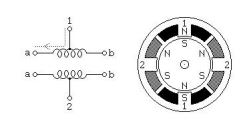
\includegraphics[scale=1]{imagens/f17}
    \caption{Motor Unipolar}
\end{figure}

\subsubsection{Motores Bipolares}

Possuem apena um único enrolamento por fase. Eles são constituídos por bobinas sem derivação central. Por este fato, estas bobinas devem ser energizadas de tal forma que a corrente elétrica flua na direção inversa a cada dois passos para permitir o movimento contínuo do rotor, ou seja, a polaridade deve ser invertida durante o funcionamento do motor. Como os enrolamentos são melhor utilizados, são mais poderosos do que um motor unipolar do mesmo peso.


\begin{figure}[ht!]
    \center 
    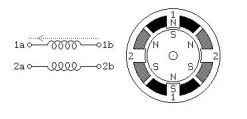
\includegraphics[scale=1]{imagens/f16}
    \caption{Motor Bipolar}
\end{figure}

\subsubsection{Ponte H}

A ponte H é um circuito do tipo chopper classe E que consegue determinar o sentido da corrente, a polaridade da tensão e a tensão em um dado sistema ou componente. O funcionamento é baseado no chaveamento de componentes eletrônicos e o módulo da tensão num dado ponto do circuito vai ser determinado usando PWM. O nome do circuito vem da forma que o mesmo é montado, onde existem quatro chaves a serem acionadas. Cada configuração faz com que o motor gire em um sentido. 

Para melhorar o circuito são utilizados diodos entre as chaves pois se a corrente não tiver onde circular, ela voltará para a fonte de alimentação e como consequência não gastará energia de uma possível bateria. Para a proteção do circuito contra curtos, utiliza-se portas lógicas com componentes 7408 e 7406. 

\begin{figure}[ht!]
    \center 
    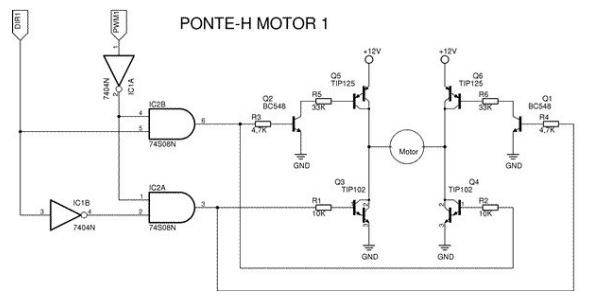
\includegraphics[scale=1]{imagens/f18}
    \caption{Ponte H}
\end{figure}

